

\begin{figure*}[t]
\centerline{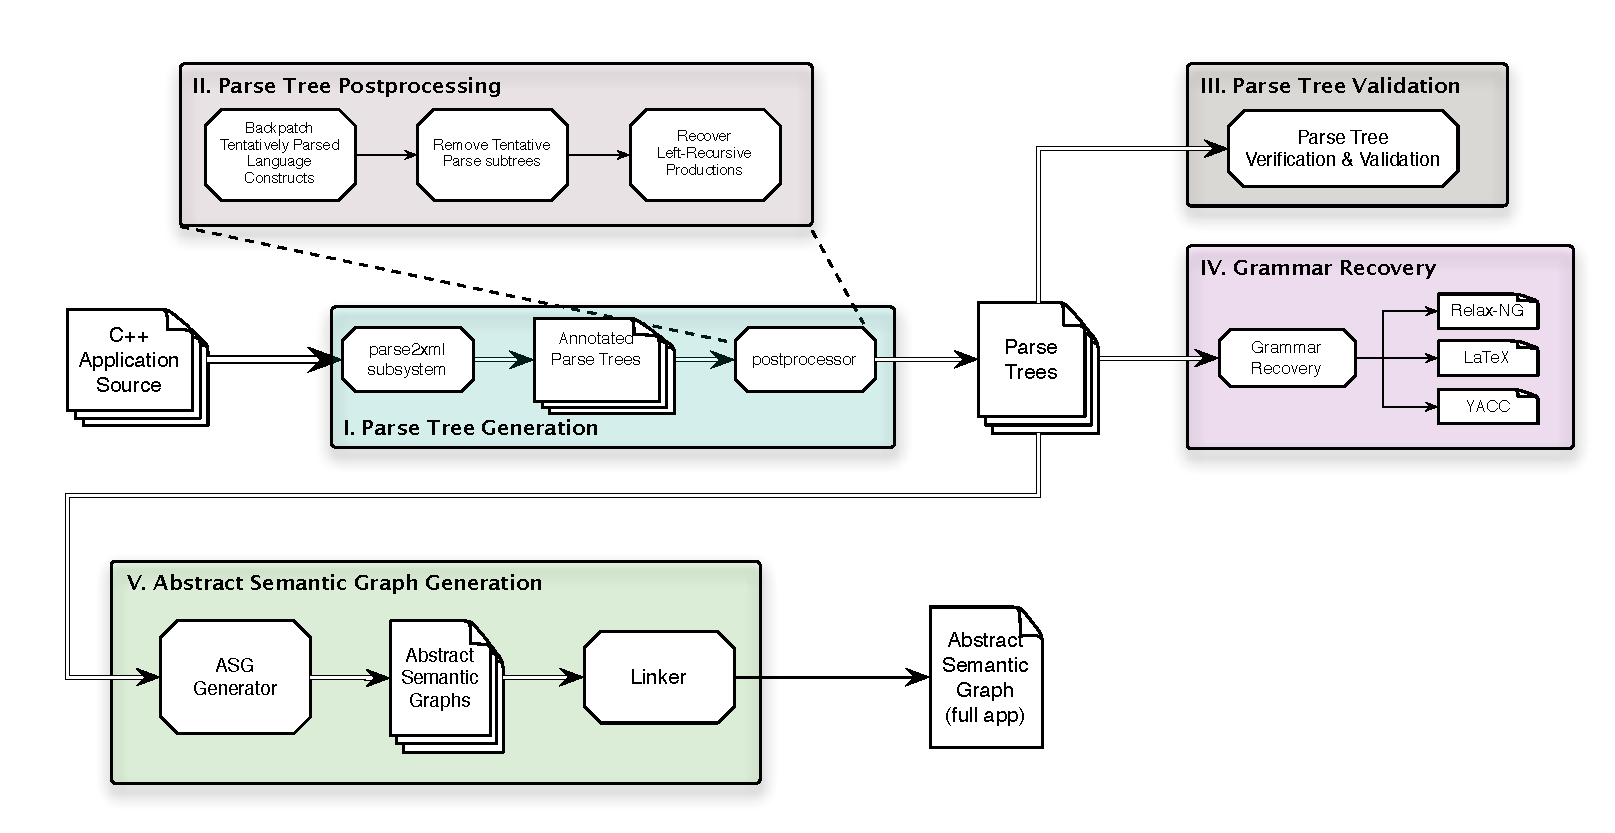
\includegraphics[scale=0.65]{figures/overview_acmse}}
\caption{{\bf \large System Summary}. This figure encapsulates the
important modules in the Hylian system.}
\label{fig:overview}
\figline
\end{figure*}


In this section, we describe Hylian, the system that we developed
to empower a researcher or developer to perform statement-level 
analysis of a program written in a gcc dialect of the {\CPP} language.
Figure \ref{fig:overview} is an overview of Hylian, which
consists of three phases: (1) Parse tree extraction and grammar
recovery, (2) development and generation of an ASG, and 
(3) transformation of the ASG.


The first phase is summarized at the top of Figure \ref{fig:overview} 
by the rectangles labeled 
I, {\sf Parse Tree Generation}; 
II, {\sf Parse Tree Postprocessing};
III, {\sf Parse Tree Validation};
and IV, {\sf Grammar Recovery}.
In module I of the first phase, we generate parse trees for each 
compilation unit in the application by augmenting the 
gcc {\CPP} parser with probes whose output generates
an XML representation for each of the respective parse trees.
The $gcc$ parser performs tentative parsing and then
backtracks to recover from incorrectly chosen alternatives. 
Thus, in module II, the parse subtrees that were emitted as part 
of an incorrect alternative are deleted and the committed subtrees 
are written to a file in XML format.
In module III, the generated parse trees are validated.
Validation entails recovery of a grammar for the gcc
{\CPP} grammar, module IV, and then use of the grammar to 
generate a schema, in Relax NG format.

The second phase, generation of an ASG, is summarized by
the two rectangles, V, {\sf Abstract Semantic Graph generation},
and VI, {\sf ASG verification}, are summarized in the middle
of Figure \ref{fig:overview}.
The focus of this paper is ASG generation, and this will
be described in more detail in Section \ref{sec:method}.


There are many advantages attached to the use of a language-complete
system, such as Hylian, the language-complete ASG 
construction system that we describe,
One of these is the subsequent feasibility of statement 
level transformations and 
subsequent code generation of the transformed ASG.
In reference \cite{IJSEKE},
We show that the use of parse trees does not provide sufficient
information to fully automate the process of generating interface
protocols for the classes in a library and that using the 
language-complete Hylian ASG, the process can be fully automated and, 
in fact, there are even more benefits of using a Hylian ASG.
However, a full explanation of these additional features is
beyond the scope of this paper.


